% vim: textwidth=99 spell spelllang=en_gb:
% chktex-file 36

\documentclass[nobib, a4paper, twoside, justified]{tufte-book}

\usepackage[utf8]{inputenc}
\usepackage[british]{babel}
\usepackage{csquotes}
\usepackage[style=verbose, autocite=footnote, backend=biber]{biblatex}

\title{Displaying Heraldic Blazons}
\author{William Mathewson}
\publisher{University of Edinburgh}
\date{January 2018}

\addbibresource{bibliography.bib}

%%%%
%%
%% LOCALS are in `tufte-book-local.tex'

\usepackage{graphicx} % allow embedded images
\setkeys{Gin}{width=\linewidth,totalheight=\textheight,keepaspectratio}
\graphicspath{{graphics/}} % set of paths to search for images
\DeclareGraphicsExtensions{.pdf,.png}

\usepackage{amsmath}  % extended mathematics
\usepackage{booktabs} % book-quality tables
\usepackage{units}    % non-stacked fractions and better unit spacing
\usepackage{multicol} % multiple column layout facilities
\usepackage{fancyvrb} % extended verbatim environments
\usepackage{amsmath}
\usepackage{xspace}
\usepackage{makeidx}
\usepackage{mathtools}

\usepackage{float}
\usepackage{subfig}

\usepackage[final]{pdfpages}

%% Tell hyperref package it may break long URLs however it feels
\usepackage{hyperref}
\def\UrlBreaks{\do\/\do-}

%\newcommand{\dcim}{\emph{DCIM}\@\xspace}
%\newcommand{\ipam}{\emph{IPAM}\@\xspace}
%\newcommand{\dcimipam}{\emph{DCIM \& IPAM}\@\xspace}
%\newcommand{\desired}{\emph{desired}\@\xspace}
%\newcommand{\operational}{\emph{operational}\@\xspace}
%\newcommand{\wikid}{\textsc{WikiD}\@\xspace}
%\newcommand{\pywikid}{\textit{pywikid}\@\xspace}
\newcommand{\code}[1]{\texttt{#1}}
%\newcommand{\pythonthree}{Python$3$\@\xspace}

\newcommand{\svg}{\gls{svg}\@\xspace}
\newcommand{\svgs}{\glspl{svg}\@\xspace}
\newcommand{\dom}{\gls{dom}\@\xspace}

\newcommand{\charge}{\gls{charge}\@\xspace}
\newcommand{\charges}{\glspl{charge}\@\xspace}
\newcommand{\tincture}{\gls{tincture}\@\xspace}
\newcommand{\tinctures}{\glspl{tincture}\@\xspace}

%\newcommand{\defeq}{\stackrel{\mathclap{\normalfont\mbox{def}}}{=}}
%\newcommand{\namedmap}[1]{\stackrel{\mathclap{\mbox{\small#1}}}{\longmapsto}}

%% R_{x->y} style
%\newcommand{\relate}[3]{\text{\itshape#1 }_{#2\ \mapsto\ #3}}

%% x --R--> y style
%\newcommand{\relate}[3]{#2\namedmap{#1}#3}

%% xRy style
%\newcommand{\relate}[3]{_{#2}#1_{#3}}

%\newcommand{\citetodo}{\sidenote{\todo{[Citation Needed]}}\@\xspace}
%\newcommand{\reftodo}{\sidenote{\todo{[Reference Needed]}}\@\xspace}
%\newcommand{\prooftodo}{\sidenote{\todo{[Substantiation Needed]}}\@\xspace}
\newcommand{\todo}[1]{{\noindent\textcolor{Red}{\textit{\quad#1}}\par}}

\let\lines\baselineskip{}

\usepackage{glossaries}
\setacronymstyle{long-short}

\loadglsentries{glossary}

\glstoctrue{}

\begin{document}

\frontmatter

\maketitlepage{}

%\abstract{This is an example of {\tt infthesis} style. The file {\tt
%skeleton.tex} generates this document and can be used to get a ``skeleton''
%for your thesis. The abstract should summarise your report and fit in the
%space on the first page.
%%
%You may, of course, use any other software to write your report, as long as
%you follow the same style. That means: producing a title page as given here,
%and including a table of contents and bibliography.  }

\begin{publicationmeta}
  \section*{Acknowledgements}
  I would like to thank my supervisor, Julian Bradfield, for his help and advice as I was writing
  this project. I would also like to thank all my friends on Level 9 of Appleton Tower who helped
  keep me going through the long, arduous journey that was this project and 4\textsuperscript{th}
  year as a whole.

  \section*{Declaration}
  I declare that this thesis was composed by myself,
  that the work contained herein is my own
  except where explicitly stated otherwise in the text,
  and that this work has not been submitted for any other degree or
  professional qualification except as specified.\par
  ({\textit{\thanklessauthor}})
\end{publicationmeta}

\tableofcontents

%\pagenumbering{Arabic}

\mainmatter{}

\chapter{Introduction}\label{cha:introduction}

This project was written as a paired project and as such I only wrote the side of the project that
deals with rendering the \glspl{blazon}, having been parsed by the back end. The back-end was
written by my partner, Anthony Gallagher, and the writing of it will not be covered in this report.
Important shared design elements will be covered however in Section~\ref{sec:core_concepts}.

\section{Motivation}\label{sec:motivation}

In 1874 --- 4 years after his death --- John Papworth's \textit{Ordinary of British Armorials} was
published~\autocite{collins_1942}. In this work, he recorded approximately 50,000 entries of
descriptions of families' coats of arms, none annotated.

This honours project would make it possible to have these descriptions, or \textit{\glspl{blazon}}
as they are termed in heraldry (see~\ref{sec:heraldry}), drawn freely for people to view. This has
potential application for ancestry companies that build family trees for people. Given the blazon,
they would be able to construct the shields visually.

\section{Contributions}\label{sec:contributions}

In this honours project, my contributions included:

\begin{itemize}
  \item Drawing the \charges{} and quarters used on the shield, or \textit{\gls{escutcheon}},
  \item Writing the base web server and
  \item Writing the quarter and \charge{} drawing algorithm
\end{itemize}

\chapter{Background}\label{cha:background}

\section{Heraldry}\label{sec:heraldry}

Many families, countries and organisations --- primarily in Europe --- have coats of arms. Coats of
arms were initially used on shields on the battlefield to identify individual knights, but later
came to be used as flags and banners for individuals and families of the upper class at court. The
Royal Coat of Arms of the United Kingdom, belonging to the British monarch, can be seen in
Figure~\ref{fig:royal_coa}. If the reader wishes to learn more about Heraldry and its history, I
would recommend to you the many heraldic works of Charles Boutell and John Brooke-Little.

\begin{marginfigure}
  \centering
  \def\svgwidth{0.8\linewidth}
  \input{graphics/Royal_Coat_of_Arms_of_the_United_Kingdom.pdf_tex}
  \caption{The Royal Coat of Arms of the United Kingdom.
  Source:~\url{https://upload.wikimedia.org/wikipedia/commons/9/98/Royal_Coat_of_Arms_of_the_United_Kingdom.svg}}%
  \label{fig:royal_coa}
\end{marginfigure}

At the centre of a coat of arms is a shield known as an \textit{escutcheon}. The language used to
describe how the escutcheon is to be drawn is known as a \textit{blazon}. Blazons have been used
since the Norman conquest and have been refined to a regular language in the
process~\autocite{boutell_1864}, although, as John Brooke-Little said, ``many of the supposedly
hard and fast rules laid down in heraldic manuals [including those by heralds] are often
ignored.''~\autocite{brooke_little_1985} This flagrant disregard for the rules introduces
difficulty in parsing the blazons as the language loses some of its regularity.

\begin{marginfigure}
  \centering
  \def\svgwidth{0.8\linewidth}
  \input{graphics/Blason_Albert.pdf_tex}
  \caption{The shield of the town of Albert, France. \textit{Barry of ten argent and
  gules}. Source:~\url{https://en.wikipedia.org/wiki/File:Blason_Albert.svg}}\label{fig:blason_albert}
\end{marginfigure}

Blazons have a few key attributes:
\begin{itemize}
  \item The \textit{\gls{field}}, which is the background colour of the shield or quarter;
  \item \textit{Ordinaries}, which are geometric shapes (as seen in Figure~\ref{fig:scrope},
    bearing a golden slash, or \textit{bend});
  \item \textit{\Glspl{charge}}, which are small emblems, such as fleur-de-lis and lions;
  \item \textit{\Glspl{variation}}, which describe how the field or \charge{} is patterned.
    \Glspl{variation} can indicate patterns such as chequered or coloured lines (as seen in
    Figure~\ref{fig:blason_albert}); and
  \item \textit{\Glspl{tincture}}, which are the colours and patterns for \charges{}, ordinaries
    and fields.
\end{itemize}

The tinctures are derived from Norman French and are divided into 3 groups, typically known as
\textit{metals}, \textit{colours} and \textit{furs}. In British heraldry, the colours are also
derived from Norman French and so the names appear archaic. In heraldry, blue is \textit{azure} and
red is \textit{gules} for instance. The metals are \textit{or} and \textit{argent}, for gold and
silver respectively. Whilst the tinctures are linked to colours, the College of Arms does not
specify which shade of that colour is required for the tinctures, leaving it to the artist to
decide~\autocite{college_of_arms_faq}. In this case, I have used default CSS colours.

\begin{marginfigure}
  \centering
  \def\svgwidth{0.8\linewidth}
  \input{graphics/chief_example.pdf_tex}
  \caption{\textit{Purpure, a chief Gules}.}\label{fig:chief_example}
\end{marginfigure}

Blazons conventionally follow a form of starting with the \textit{tincture} or \textit{variation}
of the field. After the description of the field, \textit{ordinaries} and \textit{\charges{}} are
named with their tinctures. An example of this is ``\textit{Purpure, a chief Gules}''. This blazon
describes an escutcheon with a field of \textit{purpure} (purple), with a \textit{Chief} ordinary
--- a bar across the top of the shield --- of \textit{gules} (red). This can be seen --- drawn by
the web app --- in Figure~\ref{fig:chief_example}.

\begin{marginfigure}
  \centering
  \def\svgwidth{0.8\linewidth}
  \input{graphics/scrope.pdf_tex}
  \caption{The Scrope escutcheon; \textit{Azure, a bend Or}.}\label{fig:scrope}
\end{marginfigure}

A simple --- but notable --- blazon is that of the Scrope family. In the 14th century, the Baron
Scrope brought a case action against Sir Roberts Grosvenor when he noticed that they both had the
same coat of arms. Many witnesses gave evidence in the case, including Geoffrey
Chaucer~\autocite{scrope_grosvenor}. The case was ultimately decided in Scrope's favour. The Scrope
coat of arms has a blazon of \textit{Azure, a bend Or}; a depiction of this (as drawn by the web
app written for this project) can be seen in Figure~\ref{fig:scrope}.

Whilst the Scrope arms are prominent in heraldry, they are simplistic and indicative of
medi\ae{}val arms. Coats of arms became more complex as they developed through the centuries, with
instances of \textit{quarterly} shields, \textit{grand-quarterlies} --- quarterlies within
quarterlies --- and \textit{differenced} arms. \textit{Differenced} arms involve adding an
\textit{ordinary} over an existing coat of arms. This was typically used to differentiate similar
looking coats of arms, especially between father and sons. Common examples of differentiated
shields are seen in duchies' coats of arms, particularly those which were given to Charles II's
illegitimate children. Examples of more complex shields can be seen in
Figure~\ref{fig:complex_shields}.

\begin{figure*}[h]
  \subfloat[Neville, 16th Earl of Warwick's coat of arms. An example of grand-quarterlies and
  differenced arms. Source:~\url{https://en.wikipedia.org/wiki/File:Neville_Warwick_Arms.svg}.]{%
    \def\svgwidth{0.3\linewidth} %
    \input{graphics/Neville_Warwick_Arms.pdf_tex}
  }
  \qquad
  \subfloat[A quarterly shield drawn by the web app. \textit{Quarterly: 1st and 4th: Gules, a bend
  Sable; 2nd and 3rd: Azure, a chief Or}. ]{%
    \def\svgwidth{0.28\linewidth}
    \input{graphics/quarterly_example.pdf_tex}
  }
  \caption{Some examples of more complex coats of arms.}\label{fig:complex_shields}
\end{figure*}

For a time, it was considered bad form to repeat a \textit{tincture} in a blazon, and use a
reference to the tincture's previous use. The Heraldic Society gives an example as such:
``\textit{`Azure on a fess argent three billets azure'} [would have been written as] \textit{`Azure
on a fess argent three billets of the first'}''. The `\textit{of the first}' refers to the field's
tincture of azure. This blazon describes a blue shield, with a white bar horizontally across the
middle with 3 white rectangles arranged along the bar. The Heraldic Society advocates repeating
tinctures to reduce ambiguity~\autocite{blazon_in_coa}.

\section{Related Works}%
\label{sec:related_works}

\todo{Add more related works}

Whilst many escutcheons have been drawn and uploaded to WikiMedia in
\svg~\autocite{ferraiolo2000scalable} format (some of which have been used in this report), many
appear to have been created in Inkscape~\autocite{inkscape}, rather than being created
programmatically. Much work has been done in collecting and cataloguing blazons themselves ---
namely John Papworth as mentioned in Section~\ref{sec:motivation}.

\section{Summary}%
\label{sec:background_summary}

In this chapter, we covered basic heraldry, including core terminology, as well as works related to
the project. Core heraldry terminology includes:

\begin{itemize}
  \item \textit{\Gls{escutcheon}} --- the shield in the coat of arms;
  \item \textit{\Gls{field}} --- the background of the escutcheon;
  \item \textit{\Glspl{ordinary}} --- geometric shapes on the escutcheon;
  \item \textit{\Glspl{charge}} --- small emblems, such as fleur-de-lis and lions; and
  \item \textit{\Gls{tincture}} --- the colours and patterns for \charges{}, ordinaries and fields.
\end{itemize}

All relevant heraldry terminology may be found in the Glossary on page~\pageref{glossary}.

\chapter{Design}%
\label{cha:design}

\section{Core Concepts}%
\label{sec:core_concepts}

The two languages chosen for implementing this project were Python and
TypeScript~\autocite{typescript}. Python seemed like an obvious choice with its good support for
\gls{nlp} through the \gls{nltk}~\autocite{bird2004nltk}. TypeScript is a typed superset of
JavaScript written by Microsoft that compiles, or \textit{\glspl{transpile}}, to plain JavaScript.
TypeScript was chosen as a nicer alternative to programming in pure JavaScript, thanks to the
addition of powerful features such as types, access control and abstract classes.

The core design for this project centred around having a split stack; with a Python back-end
parsing the blazon, serialising it into JSON \marginnote{\gls{json} is a lightweight
  data-interchange format, consisting of key-value pairs, array data types and other serialisable
  data types (such as strings, numbers and booleans). JSON is derived from JavaScript's associative
array-style data type, \texttt{Object}. An example of JSON can be seen in
Figure~\ref{fig:expected_output}.} and passing it to the TypeScript front-end, which then drew it
onto the webpage. This allowed for large amounts of flexibility, enabling the two halves of the
project to be developed in tandem with the Separation of Concerns principle being adhered to
throughout. It also allows for pluggable rendering implementations as the JSON schema for drawing
payloads can be well-defined.

The Python back-end received a JSON payload from the webpage containing the blazon; it parsed the
blazon using a Context-Free Grammar (CFG) parser and identified the most important parts of the
blazon. It then serialised these back into a JSON response to be sent to the webpage for rendering.
The specification was such that if the webpage was given a blazon of ``Azure, a bend Or'', it would
return the JSON payload seen in Figure~\ref{fig:expected_output}.

\begin{figure}
  \begin{verbatim}
    {
      "field": "azure",
      "charges": [{
        "charge": "bend",
        "tincture": "or"
      }]
    }
  \end{verbatim}
  \caption{Expected output from the Python back end, for a given blazon of ``Azure, a bend Or''.}%
  \label{fig:expected_output}
\end{figure}

The TypeScript front-end received this payload, applied the \textit{azure} CSS class to the field
element, then drew a bend onto the field with an \textit{or} CSS class.

Escutcheons were drawn using the \svg{} format for portability across browsers as well as the
eponymous scalability of \svg{} images. This allowed drawn escutcheons to be embedded elsewhere
with ease, either directly or through rendering the \svgs{} as other image formats via programmes
like Inkscape.

\section{External Dependencies}%
\label{sec:external_dependencies}

The front-end depended on a pair of libraries for \svg{} rendering and \dom{} manipulation: the
selection library of D3.js~\autocite{d3js} and jQuery~\autocite{jquery}. D3.js provides many
powerful functions for \svg{} and \dom{} manipulation, especially creating and editing \svg{} and
HTML elements. It would also rely on jQuery for further \dom{} manipulation. The Mozilla Developer
Network defines the \dom{} as such: ``The Document Object Model (DOM) connects web pages to scripts
or programming languages. Usually that means JavaScript, but modelling HTML, SVG, or XML documents
as objects is not part of the JavaScript language. The DOM model represents a document with a
logical tree. Each branch of the tree ends in a node, and each node contains objects. DOM methods
allow programmatic access to the tree; with them you can change the document's structure, style or
content. Nodes can have event handlers attached to them. Once an event is triggered, the event
handlers get executed.''~\autocite{mdn_dom}.

For further assets, Sass~\autocite{sass-lang} was used as a CSS pre-processor and
Bootswatch~\autocite{bootswatch-flatly} was used for the base styling.  Webpack~\autocite{webpack}
was used to \gls{transpile} TypeScript down to JavaScript --- minifying and uglifying it in the
process --- and concatenate all source files and their dependencies into one main JavaScript
\textit{bundle} file. \textit{\Gls{minification}} of JavaScript assets involves stripping out all
unnecessary whitespace and tokens. \textit{\Gls{uglification}} transforms the JavaScript code by
renaming all variables and functions into short, obfuscated names to reduce the footprint of the
assets. These two techniques can decrease loading times of web apps as the browser have smaller
asset payloads to download than the original, raw source code.

\subsection{Development Dependencies}%
\label{sub:development_dependencies}

To maintain code readability and prevent bugs, TSLint~\autocite{tslint} was used and set up to
automatically run as part of the Travis \gls{ci}~\autocite{travis} service, causing a build to fail
if the linter detected a style violation. For unit testing, Jest~\autocite{jest} (with
ts-jest~\autocite{ts-jest} for TypeScript support) was used, especially for its powerful mocking
and expectation matcher functionality. Automated documentation generation was provided by
TypeDoc~\autocite{typedoc}.

\section{Iterative Design}%
\label{sec:iterative_design}

Iterative design was used as the design process for writing the code for this project. Iterative
design is a cyclical process of designing, prototyping and evaluating. One designs and prototypes a
new feature before evaluating the final feature design. If the design is acceptable, the new
feature is implemented, otherwise the cycle restarts. An iterative design process allows to address
different functionality as separate tasks, building on top of one another. It also allows to
heavily refactor a project whilst staying in one cycle.

\subsection{First Iteration}%
\label{sub:first_iteration}

The first design iteration had a specific focus on basic \charge{} drawing, with a plan to begin a
second iteration for adding quarterly rendering with lessons learnt from implementing \charge{}
drawing in the first iteration. The second design iteration is described in
Section~\ref{sub:second_design_iteration}.

I decided to have all drawing logic defined in the client, existing in a single module with minimum
dependencies. The shield outline was rendered on the page on load as part of the HTML template.
This helped support a reliable entry point for the drawing logic as it was able to easily select
the shield element to begin appending other \svg{} elements to. Appending these \svg{} elements
allowed layering to be achieved as \svg{} orders layers based on the order of elements in the
document. This was used to great effect later when drawing quarters (see
Section~\ref{sub:second_design_iteration}).

The front-end was designed around functional paradigms; breaking up major functionality into
functions that would deal with smaller, encapsulated functionality, such as adding extra layers to
the HTML template or clearing the shield when drawing a new blazon. This allowed for a stable API,
as the single point of access function would not be renamed but all other functions may be changed
and updated separately. As described in Section~\ref{sec:core_concepts}, the front-end first
accessed the \textit{field} value in the parsed JSON payload, applied the value as the CSS class
for the shield and then moved onto the \charges{}. It iterated over the \textit{\charges{}} array
in the payload, drawing each \charge{} onto the shield and applying the tincture as the CSS class.
Due to \svg{} layering, as mentioned earlier, if there were multiple \charges{} specified in the
payload, all would be drawn according to the array ordering.

\chapter{Implementation}%
\label{cha:implementation}

\section{Initial Approach}%
\label{sec:initial_approach}

As described in Section~\ref{sub:first_iteration}, the initial approach was to have all methods in
the core \texttt{index.ts} file that would be \gls{transpile}d and loaded in the browser. This
meant a smaller footprint when the code was bundled by Webpack and easier maintenance as all
relevant functions were next to one another, following the Step-Down
Rule~\autocite{martin2009clean}\footnote{The Step-Down Rule dictates that if function \texttt{A()}
calls function \texttt{B()} and \texttt{C()} in its function body, functions \texttt{A()} and
\texttt{B()} should be defined immediately after function \texttt{A()}.}.

The web app had a single entry point of \texttt{drawShield(blazon)}, where \texttt{blazon} was the
whole JSON payload returned from the \texttt{/\_parse} endpoint. (See
Figure~\ref{fig:expected_output} for an example payload.) This presented a problem initially as
TypeScript didn't handle the unstructured parsed data well due to it being a JavaScript
\texttt{Object}\footnote{In JavaScript, an \texttt{Object} works as both an associative array and a
basis for classes and inheritance through its \texttt{prototype} field.} instance. Attempting to
access members of this object (such as \texttt{field}) causes TypeScript to produce an error that
the contents might be undefined and thus return a \texttt{null} object. To fix this, I designed
\texttt{interface}s with the expected fields in the payload; one for the whole object,
\texttt{IBlazon}, and one for the \charges{} array contained within, \texttt{ICharge}. Similarly,
to avoid problems with string matching, I defined 2 \texttt{enum}s to represent the supported
tinctures and \charges{}, \texttt{ETincture} and \texttt{ECharge} respectively. As discussed in
Section~\ref{sec:adding_quarterly_rendering}, I later added another \texttt{enum} for quarters.
(All \texttt{interface}s and \texttt{enum}s can be found in
Appendix~\ref{cha:interfaces_and_enums}.) Having fixed this data problem,
\texttt{drawShield(blazon)} was now able to access members of the blazon object safely.

To avoid the problem of overlapping \charges{}, I had to write a \texttt{clearShield()} method that
would iterate over all the \texttt{path} nodes in the \svg{} block, and delete them. This, however,
promptly deleted the shield outline, so I had to add a check to prevent deleting \texttt{path}
nodes with a \texttt{\#shield} id, instead only removing the CSS class. Having cleared the shield
of any possible obstructions, the \texttt{drawShield} method would then assign the contents of the
\texttt{field} value as the CSS class and iterate over the \texttt{\charges{}} array, passing each
\charge{} to \texttt{drawCharge(charge: ICharge)}.

When each \charge{} node is created in \texttt{drawCharge}, it is assigned an id. This id is formed
from the name of the charge, followed by a random number in the range $1\text{--}512$ inclusive
with the hope that the range is large enough to lack overlaps.

To draw shapes in \svg{}, a \texttt{path} node requires a `\texttt{d}' attributes which contains
the commands for drawing said shape. To generate all these attributes, I drew all the \charge{}
shapes in Inkscape and extracted the `\texttt{d}' attribute from the generated \svgs{}. At first, I
put a \texttt{Map}\footnote{A \texttt{Map} here is a TypeScript/JavaScript data type, also known as
a \texttt{HashMap} or an associative array} of the \charges{} and their paths in the global scope,
available for all functions to access. This worked for \charges{} that were produced using a
\texttt{path} node with a `\texttt{d}' attribute, but introduced problems when using the
\textit{chief} \charge{} (a chief \charge{} being displayed in Figure~\ref{fig:chief_example}). The
chief \charge{} was drawn using a \texttt{rect} node which required `\texttt{x}' and `\texttt{y}'
co-ordinates to specify a starting point and \texttt{height} and \texttt{width} attributes to
describe the size of the rectangle. To address this, I wrote a \texttt{ChargeShapes} class to
encapsulate the \charges{} and their attributes. This class provided one public member,
\texttt{chargePaths} which was of the type \texttt{Map<string, Map<string, string>\hphantom{}>}.
Having this as a map allowed \texttt{drawCharge} to first check if the app knew how to draw the
\charge{} by checking whether \texttt{ChargeShapes.chargePaths} contained the \charge{} as a key.
If the \charge{} had an entry, then \texttt{drawCharge} would iterate over the attribute
\texttt{Map} and apply them to the \texttt{path} or \texttt{rect} node, before finally applying the
CSS class.

\begin{marginfigure}
  \centering
  \def\svgwidth{0.8\linewidth}
  \input{graphics/sinister_example.pdf_tex}
  \caption{\textit{Or, a bend sinister Vert.}}\label{fig:sinister_example}
\end{marginfigure}

The final part of \texttt{drawCharge} applied a transform to the \texttt{path} if the payload
included a boolean flag \texttt{sinister} to indicate that the bend \charge{} should be flipped.
This writes to an attribute \texttt{transform} which applies a \texttt{matrix} transformation that
flips the \charge{} followed by a \texttt{translate} transformation to move it into place. An
example of a sinister bend can be seen in Figure~\ref{fig:sinister_example}.

Whilst this simple implementation worked well for drawing basic \glspl{escutcheon}, like
Figure~\ref{fig:chief_example} and Figure~\ref{fig:sinister_example}, it wasn't able to draw more
complex shields like those seen in Figure~\ref{fig:complex_shields}.

\section{Adding Quarterly Rendering}%
\label{sec:adding_quarterly_rendering}

\subsection{Replanning to Refactor}%
\label{sub:replanning_to_refactor}

Whilst prototyping for adding functionality to render quarterly shields, I found that it was going
to be impossible to maintain the initial, atomic design laid out in
Section~\ref{sec:initial_design} whilst also keeping the code clean and readable. To counter this,
I designed a new, modular system that leaned more heavily into Object-Oriented paradigms than
functional ones. All major sections of functionality, including \gls{blazon} parsing, \charge{} and
quarter rendering, were encapsulated in their own class with clear names and well-defined, shared
APIs. This new design was written to follow the SOLID~\autocite{martin2000design} object-oriented
design principles where possible.

\subsection{SOLID Design Principles}%
\label{sub:solid_design_principles}

\todo{Refactor all this, see photos, break principles into relevant sections.}

SOLID object-oriented design is a collection of 5 design principles:

\begin{itemize}
  \item \textit{The Single Responsibility Principle} --- a class should have one, and only one,
    reason to change;
  \item \textit{The Open Closed Principle} --- you should be able to extend a class's behaviour,
    without modifying it;
  \item \textit{The Liskov Substitution Principle} --- derived classes must be substituable for
    their base classes;
  \item \textit{The Interface Segregation Principle} --- make fine grained interfaces that are
    client specific and
  \item \textit{The Dependency Inversion Principle} --- depend on abstractions, not on concretions.
\end{itemize}

\section{Refactoring Charge Rendering}%
\label{sec:refactoring_charge_rendering}

\chapter{Results and Discussion}%
\label{cha:results_and_discussion}

\section{Automated Testing}%
\label{sec:automated_testing}

\section{Rendering Testing}%
\label{sec:rendering_testing}

\chapter{Conclusion}%
\label{cha:conclusion}

\section{Overview}%
\label{sec:overview}

\section{Further Work}%
\label{sec:further_work}



\backmatter%

\printbibliography[heading=bibintoc]

\printglossary%
\label{glossary}

% vim: textwidth=99 spell spelllang=en_gb:
\graphicspath{{graphics/}} % set of paths to search for images
\DeclareGraphicsExtensions{.pdf,.png}

\appendix
\setboolean{@mainmatter}{true}

\chapter{Interfaces and Enums}%
\label{cha:interfaces_and_enums}

\begin{verbatim}
enum ETincture {
  /** For specifying Quarters */
  Quarterly = "quarterly",
  /** Gold/yellow */
  Or = "or",
  /** White */
  Argent = "argent",
  /** Blue */
  Azure = "azure",
  /** Red */
  Gules = "gules",
  /** Purple */
  Purpure = "purpure",
  /** Black */
  Sable = "sable",
  /** Green */
  Vert = "vert",
}

enum ECharge {
  Bend = "bend",
  Cross = "cross",
  Chief = "chief",
  Saltire = "saltire",
}

enum EQuarter {
  TL = "quarterly_tl",
  TR = "quarterly_tr",
  BL = "quarterly_bl",
  BR = "quarterly_br",
}

interface ICharge {
  charge: ECharge;
  sinister?: boolean;
  tincture?: ETincture;
}

interface IBlazon {
  field: ETincture;
  charges: ICharge[];
}
\end{verbatim}

A question mark on a field in an \texttt{interface} denotes it as optional.

\chapter{UML Diagrams}%
\label{cha:uml_diagrams}

In these UML diagrams, \texttt{d3.Selection} is a data type defined by D3.js~\autocite{d3js}. It
contains a reference to an HTML element for use in \dom{} manipulation.

\section{Second Design Iteration Diagrams}%
\label{sec:second_design_iteration_diagrams}

\begin{figure*}[h]
  %\centering
  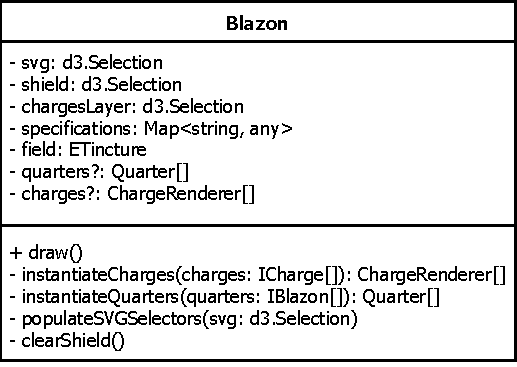
\includegraphics[width=0.5\linewidth]{BlazonUML}
  \caption{\texttt{Blazon} UML.}%
  \label{fig:BlazonUML}
\end{figure*}

\begin{figure*}[h]
  %\centering
  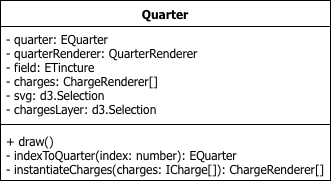
\includegraphics[width=0.5\linewidth]{QuarterUML}
  \caption{\texttt{Quarter} UML.}%
  \label{fig:QuarterUML}
\end{figure*}

\begin{figure*}[h]
  %\centering
  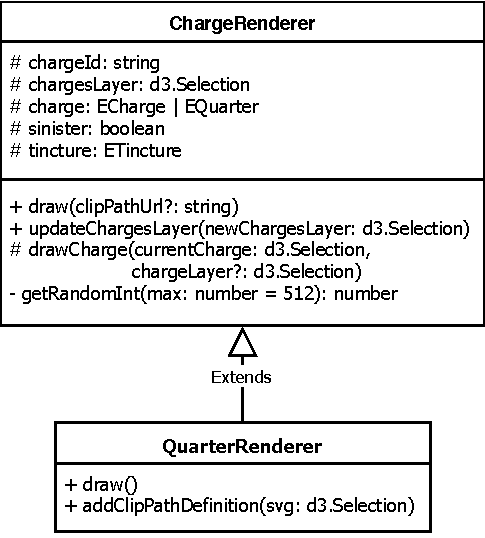
\includegraphics[width=0.5\linewidth]{ChargeRendererUML}%
  \caption{\texttt{ChargeRenderer} hierarchy and methods.}%
  \label{fig:charge_renderer_hierarchy}
\end{figure*}

\pagebreak%

\section{Third Design Iteration Diagrams}%
\label{sec:third_design_iteration_diagrams}

\begin{figure*}[h]
  %\centering
  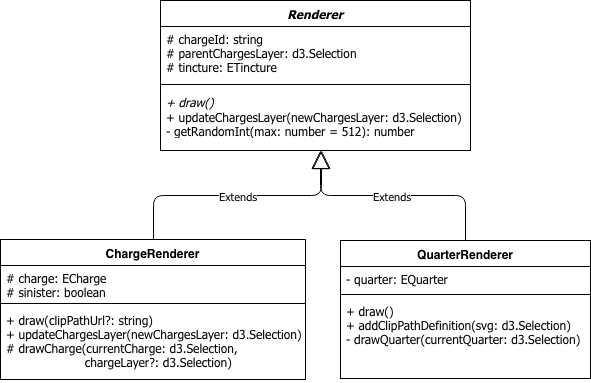
\includegraphics[width=0.8\linewidth]{RendererUML}
  \caption{\texttt{Renderer} hierarchy and methods.}%
  \label{fig:RendererUML}
\end{figure*}

\begin{figure*}[h]
  %\centering
  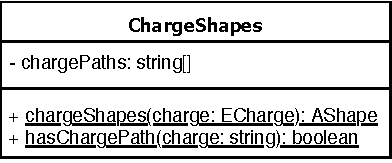
\includegraphics[width=0.5\linewidth]{ChargeShapesUML}
  \caption{\texttt{ChargeShapes} UML.}%
  \label{fig:ChargeShapesUML}
\end{figure*}

\begin{figure*}[h]
  %\centering
  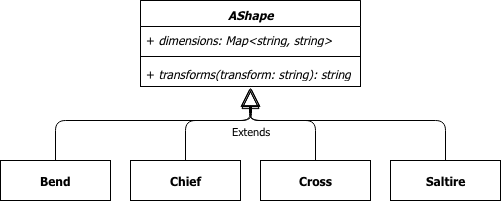
\includegraphics[width=0.8\linewidth]{AShapeUML}
  \caption{\texttt{AShape} hierarchy and methods.}%
  \label{fig:AShapeUML}
\end{figure*}

\setboolean{@mainmatter}{false}


\end{document}
